\section{Modelul informaţional de bază - ONF TR-512.1}

Modelul informațional de bază, \textit{CoreModel} reprezintă o recomandare făcută de grupul \textit{Information Modeling} din cadrul \gls{onf}. Aceasta propune un model care să descrie resursele din planul de date al unei rețele de transport, indiferent de tehnologia folosită, cu scopul de a fi folosit în activitățile de control și administrare.

Un model informațional descrie lucrurile dintr-un domeniu, în ceea ce priveşte obiectele, proprietăţile lor (reprezentate prin atribute) și relaţiile dintre acestea \cite{onftr512v1.0}. Scopul dezvoltării unui astfel de model este acela de a fi folosit de către echipamentele de control \gls{sdn}, pentru administrarea automată a unor astfel de rețele de transport, în concordanţă cu arhitectura \gls{sdn}. Echipamentul de control va prezenta cu ajutorul acestui model viziunea sa asupra rețelei către clienţii acestuia (care pot fi aplicații software sau alte echipamente de control).

\textit{CoreModel} propune obiecte de bază care reprezintă planul de date al unei rețele, care sunt însă independente de tehnologia folosită pentru transportul datelor. Acestea pot fi apoi folosite pentru dezvoltarea de modele informaționale specifice pentru anumite tehnologii (de exemplu tehnologii fără fir - microunde sau unde milimetrice, tehnologii optice, etc.). Modelul conține și obiecte care pot fi folosite în aplicații specifice, însă toate acestea sunt independente de protocoalele care ar putea fi folosite în planul de control. El este propus în limbajul \gls{uml} și se bazează și pe alte modele informaționale, propuse de alte organizaţii care dezvoltă standarde.

\begin{figure}[t]
	\centering
	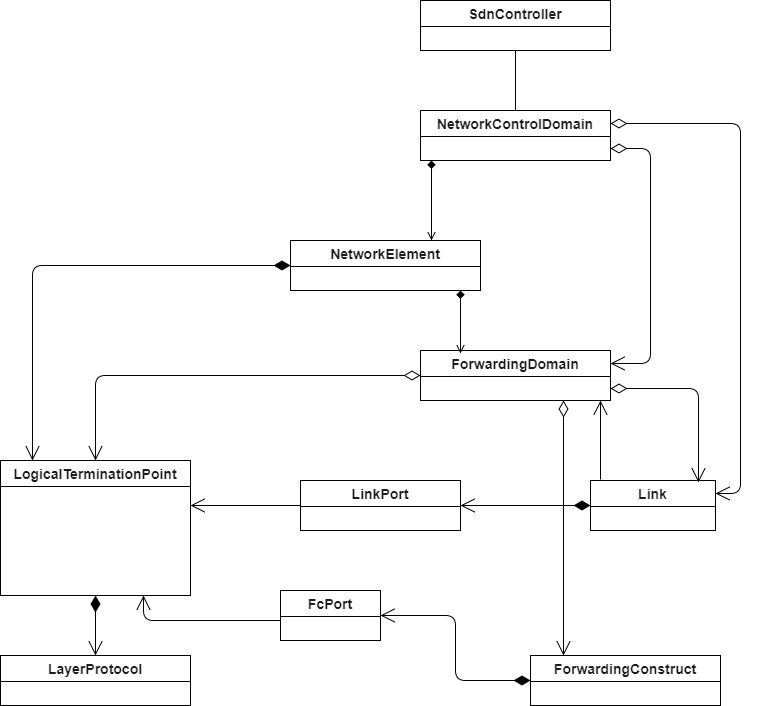
\includegraphics[width=1\textwidth]{core_model_uml_overview}
	\caption{Reprezentare UML simplificată a \textit{CoreModel}}
	\label{fig:core_model}
\end{figure}

O vedere de ansamblu simplificată, folosind \gls{uml} se poate vedea în Figura \ref{fig:core_model}. Blocurile relevante pentru simulatoarele dezvoltate vor fi detaliate în paragrafele următoare.

\subsection{Network Element}

\subsection{Forwarding Domain}

\subsection{Forwarding Construct}

\subsection{FC Port}

\subsection{Logical Termination Point}

\subsection{Layer Protocol}